\documentclass[a4paper,10pt]{report}\input{../0.Préambule/Préambule_cours_prof}\begin{document}

\pagestyle{empty}
\newpage
\noindent NOM, Prénom et classe : \dotfill

\section*{Espace : Pavé et solides}
\addcontentsline{toc}{section}{Espace : Pavé et solides}

\noindent \textit{L'usage de la calculatrice est \textbf{interdite}.} \hfill \textit{Durée : 30 minutes}

\medskip
\paragraph{Exercice 1}: \hfill \textbf{4 points}

Observer le pavé droit représenté ci-contre et compléter :

\noindent \begin{minipage}{10.5cm}
\begin{enumerate}
\item Quelle est :
\begin{enumerate}
\item La nature de la face $FGHE$ en réalité et sur le dessin : 

\medskip
\dotfill

\medskip
\dotfill
\item La nature de la face $BCHG$ en réalité et sur le dessin :

\medskip
\dotfill

\medskip
\dotfill
\end{enumerate}
\end{enumerate}
\end{minipage}
\begin{minipage}{7cm}
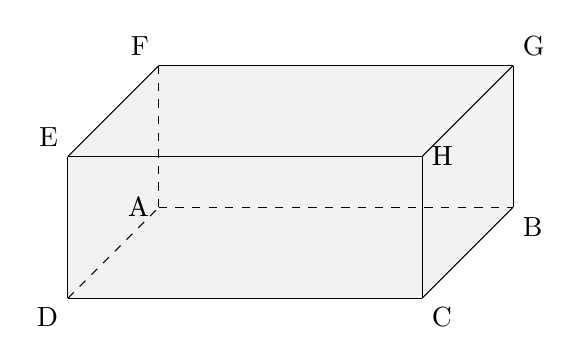
\begin{tikzpicture}[join=round,x=0.9cm,y=0.9cm,scale=1]
\tikzstyle{conefill} = [fill=gray!20,fill opacity=0.3]
%coordonnées des sommets   
%base inférieure
\draw(0,0,0)node[left](A){A};
\draw(5,0,0)node[below right](B){B};
\draw(5,0,3)node[below right](C){C};
\draw(0,0,3)node[below left](D){D};
%base supérieure
\draw(0,2,0)node[above left](E){F};
\draw(5,2,0)node[above right](F){G};
\draw(5,2,3)node[right](G){H};
\draw(0,2,3)node[above left](H){E}; 
%remplir les faces
\fill[conefill] (0,0,0)--(5,0,0)--(5,0,3)--(0,0,3)--cycle; %base inférieure
\fill[conefill] (0,2,0)--(5,2,0)--(5,2,3)--(0,2,3)--cycle; %base supérieure
\fill[conefill] (0,0,0)--(0,2,0)--(0,2,3)--(0,0,3)--cycle; %face latérale gauche
\fill[conefill] (0,0,0)--(5,0,0)--(5,2,0)--(0,2,0)--cycle; %face arrière
\fill[conefill] (5,0,0)--(5,2,0)--(5,2,3)--(5,0,3)--cycle; %face latérale droite
\fill[conefill] (0,0,3)--(5,0,3)--(5,2,3)--(0,2,3)--cycle; %face avant 
%tracer les arêtes
\draw[dashed]  (A.east)--(B.north west);
\draw[dashed]  (D.north east)--(A.east);
\draw[dashed] (A.east)--(E.south east);
%tracer les arêtes
\draw (B.north west)-- (C.north west);
\draw (C.north west)-- (D.north east);
\draw (E.south east)--(F.south west);
\draw (F.south west)--(G.west);
\draw (G.west)--(H.south east);
\draw (H.south east)--(E.south east);
\draw (B.north west)--(F.south west);
\draw (C.north west)--(G.west);
\draw (D.north east)-- (H.south east); 
\draw(5,2,3)node[right](G){H};
\draw(0,0,0)node[left](A){A}; 
\end{tikzpicture}
\end{minipage}


\begin{enumerate}
\setcounter{enumi}{1}
\item Citer :
\begin{enumerate}
\item une arête perpendiculaire à l'arête $[AD]$ :\medskip
\dotfill

\item la face opposée à la face $ABGF$ :\medskip
\dotfill

\item Deux arêtes de même longueur que l'arête $[GF]$ :\medskip
\dotfill
\end{enumerate} 
\end{enumerate}


\medskip
\paragraph{Exercice 2}: \hfill \textbf{2 points}

\medskip
\medskip
Voici le patron d'un pavé droit. 

\noindent Compléter les longueurs manquantes sur chaque flèche.

\vspace{-1.3cm}
\begin{flushright}

\includegraphics[scale=0.4]{../40.Image/DS5 Espace 1.png} \hspace{2cm}.
\end{flushright}

\medskip
\paragraph{Exercice 3}: \hfill \textbf{4 points}

Compléter les vues en perspective cavalière des pavés droits suivants :

\begin{center}
\begin{tikzpicture}[line cap=round,line join=round,>=triangle 45,x=0.5cm,y=0.5cm]
\draw [color=lightgray, xstep=0.5cm,ystep=0.5cm] (-3.,-3.) grid (26.,10.);
\clip(-3.,-3.) rectangle (26.,10.);
\draw [line width=2.pt] (2.,0.)-- (2.,5.);
\draw [line width=2.pt] (2.,5.)-- (5.,7.);
\draw [line width=2.pt] (2.,5.)-- (6.,5.);
\draw [line width=2.pt] (21.,7.)-- (15.,7.);
\draw [line width=2.pt] (15.,7.)-- (19.,5.);
\draw [line width=2.pt] (19.,5.)-- (19.,0.);
\begin{scriptsize}
\end{scriptsize}
\end{tikzpicture}
\end{center}

\newpage
\paragraph{Exercice 4}: \hfill \textbf{5 points}

\begin{center}
\renewcommand{\arraystretch}{1.3}
\begin{tabularx}{\linewidth}{|c|m{6cm}|*{3}{>{\centering \arraybackslash}X|}c|}\hline
&&\textbf{A}&\textbf{B}&\textbf{C} & Réponse \\ \hline

1& Un pavé droit a ... & $8$ sommets et $6$ faces & $6$ faces et $10$ arêtes & $12$ arêtes et $4$ sommets &\\ \hline

2&La base d'un cone est ... & Un triangle & Un cylindre & Un disque & \\ \hline
3&Combien d'arêtes possède une pyramide à base triangulaire ... & $6$ & $4$ & $8$ &\\ \hline
4& Quelle est la nature de ce solide représenté en perspective cavalière \begin{center}

\includegraphics[scale=0.8]{../40.Image/DS5 Espace 3.png}
\end{center}& Un prisme droit & Un pavé droit & Un cylindre & \\\hline
5& A quel solide ce patron est-il associé \begin{center}

\includegraphics[scale=0.8]{../40.Image/DS5 Espace 4.png}
\end{center}& Une pyramide & Un prisme droit à base triangulaire & Un prisme droit à base rectangulaire & \\\hline
6& Lequel de ces patrons dessinés représente un cube ? & \begin{center}

\includegraphics[scale=0.6]{../40.Image/DS5 Espace 5.1.png}
\end{center} & \begin{center}

\includegraphics[scale=0.6]{../40.Image/DS5 Espace 5.2.png}
\end{center} & \begin{center}

\includegraphics[scale=0.6]{../40.Image/DS5 Espace 5.3.png}
\end{center} & \\\hline
7& Combien de bases possède ce solide \begin{center}

\includegraphics[scale=0.4]{../40.Image/DS5 Espace 6.png}
\end{center}& $6$ & $2$ &$7$ &  \\ \hline
8& Pour la représentation en perspective cavalière ci-contre, l'arête dont le dessin est incorrect est ... \quad \quad 
\includegraphics[scale=0.7]{../40.Image/DS5 Espace 7.png} & $[AB]$ & $[BF]$ & $[BC]$ & \\ \hline
9& Quel solide a deux bases mais aucun sommet : & Le cône & Le cylindre & La sphère & \\ \hline
10& Combien de faces possède le solide suivant \begin{center}

\includegraphics[scale=0.6]{../40.Image/DS5 Espace 8.png}
\end{center} & $8$  &  $10$ & $5$ & \\ \hline
\end{tabularx}
\end{center}

\newpage
\paragraph{Exercice 5}: \hfill \textbf{4 points}

\medskip
\medskip
En utilisant le quadrillage, construire le patron du pavé droit suivant :
\begin{center}


\includegraphics[scale=1]{../40.Image/DS5 Espace 2.png}
\end{center}


\begin{center}
\noindent\petitscarreaux{16.5cm}{15cm}
\end{center}

\newpage

\paragraph{Page de recherche }

\begin{center}
\noindent\petitscarreaux{16.5cm}{10cm}
\end{center}

\end{document}